% Options for packages loaded elsewhere
\PassOptionsToPackage{unicode}{hyperref}
\PassOptionsToPackage{hyphens}{url}
\PassOptionsToPackage{dvipsnames,svgnames,x11names}{xcolor}
%
\documentclass[
  letterpaper,
  DIV=11,
  numbers=noendperiod]{scrartcl}

\usepackage{amsmath,amssymb}
\usepackage{iftex}
\ifPDFTeX
  \usepackage[T1]{fontenc}
  \usepackage[utf8]{inputenc}
  \usepackage{textcomp} % provide euro and other symbols
\else % if luatex or xetex
  \usepackage{unicode-math}
  \defaultfontfeatures{Scale=MatchLowercase}
  \defaultfontfeatures[\rmfamily]{Ligatures=TeX,Scale=1}
\fi
\usepackage{lmodern}
\ifPDFTeX\else  
    % xetex/luatex font selection
\fi
% Use upquote if available, for straight quotes in verbatim environments
\IfFileExists{upquote.sty}{\usepackage{upquote}}{}
\IfFileExists{microtype.sty}{% use microtype if available
  \usepackage[]{microtype}
  \UseMicrotypeSet[protrusion]{basicmath} % disable protrusion for tt fonts
}{}
\makeatletter
\@ifundefined{KOMAClassName}{% if non-KOMA class
  \IfFileExists{parskip.sty}{%
    \usepackage{parskip}
  }{% else
    \setlength{\parindent}{0pt}
    \setlength{\parskip}{6pt plus 2pt minus 1pt}}
}{% if KOMA class
  \KOMAoptions{parskip=half}}
\makeatother
\usepackage{xcolor}
\setlength{\emergencystretch}{3em} % prevent overfull lines
\setcounter{secnumdepth}{-\maxdimen} % remove section numbering
% Make \paragraph and \subparagraph free-standing
\ifx\paragraph\undefined\else
  \let\oldparagraph\paragraph
  \renewcommand{\paragraph}[1]{\oldparagraph{#1}\mbox{}}
\fi
\ifx\subparagraph\undefined\else
  \let\oldsubparagraph\subparagraph
  \renewcommand{\subparagraph}[1]{\oldsubparagraph{#1}\mbox{}}
\fi


\providecommand{\tightlist}{%
  \setlength{\itemsep}{0pt}\setlength{\parskip}{0pt}}\usepackage{longtable,booktabs,array}
\usepackage{calc} % for calculating minipage widths
% Correct order of tables after \paragraph or \subparagraph
\usepackage{etoolbox}
\makeatletter
\patchcmd\longtable{\par}{\if@noskipsec\mbox{}\fi\par}{}{}
\makeatother
% Allow footnotes in longtable head/foot
\IfFileExists{footnotehyper.sty}{\usepackage{footnotehyper}}{\usepackage{footnote}}
\makesavenoteenv{longtable}
\usepackage{graphicx}
\makeatletter
\def\maxwidth{\ifdim\Gin@nat@width>\linewidth\linewidth\else\Gin@nat@width\fi}
\def\maxheight{\ifdim\Gin@nat@height>\textheight\textheight\else\Gin@nat@height\fi}
\makeatother
% Scale images if necessary, so that they will not overflow the page
% margins by default, and it is still possible to overwrite the defaults
% using explicit options in \includegraphics[width, height, ...]{}
\setkeys{Gin}{width=\maxwidth,height=\maxheight,keepaspectratio}
% Set default figure placement to htbp
\makeatletter
\def\fps@figure{htbp}
\makeatother
\newlength{\cslhangindent}
\setlength{\cslhangindent}{1.5em}
\newlength{\csllabelwidth}
\setlength{\csllabelwidth}{3em}
\newlength{\cslentryspacingunit} % times entry-spacing
\setlength{\cslentryspacingunit}{\parskip}
\newenvironment{CSLReferences}[2] % #1 hanging-ident, #2 entry spacing
 {% don't indent paragraphs
  \setlength{\parindent}{0pt}
  % turn on hanging indent if param 1 is 1
  \ifodd #1
  \let\oldpar\par
  \def\par{\hangindent=\cslhangindent\oldpar}
  \fi
  % set entry spacing
  \setlength{\parskip}{#2\cslentryspacingunit}
 }%
 {}
\usepackage{calc}
\newcommand{\CSLBlock}[1]{#1\hfill\break}
\newcommand{\CSLLeftMargin}[1]{\parbox[t]{\csllabelwidth}{#1}}
\newcommand{\CSLRightInline}[1]{\parbox[t]{\linewidth - \csllabelwidth}{#1}\break}
\newcommand{\CSLIndent}[1]{\hspace{\cslhangindent}#1}

\usepackage{booktabs}
\usepackage{longtable}
\usepackage{array}
\usepackage{multirow}
\usepackage{wrapfig}
\usepackage{float}
\usepackage{colortbl}
\usepackage{pdflscape}
\usepackage{tabu}
\usepackage{threeparttable}
\usepackage{threeparttablex}
\usepackage[normalem]{ulem}
\usepackage{makecell}
\usepackage{xcolor}
\usepackage{siunitx}

  \newcolumntype{d}{S[
    input-open-uncertainty=,
    input-close-uncertainty=,
    parse-numbers = false,
    table-align-text-pre=false,
    table-align-text-post=false
  ]}
  
\KOMAoption{captions}{tableheading}
\makeatletter
\makeatother
\makeatletter
\makeatother
\makeatletter
\@ifpackageloaded{caption}{}{\usepackage{caption}}
\AtBeginDocument{%
\ifdefined\contentsname
  \renewcommand*\contentsname{Table of contents}
\else
  \newcommand\contentsname{Table of contents}
\fi
\ifdefined\listfigurename
  \renewcommand*\listfigurename{List of Figures}
\else
  \newcommand\listfigurename{List of Figures}
\fi
\ifdefined\listtablename
  \renewcommand*\listtablename{List of Tables}
\else
  \newcommand\listtablename{List of Tables}
\fi
\ifdefined\figurename
  \renewcommand*\figurename{Figure}
\else
  \newcommand\figurename{Figure}
\fi
\ifdefined\tablename
  \renewcommand*\tablename{Table}
\else
  \newcommand\tablename{Table}
\fi
}
\@ifpackageloaded{float}{}{\usepackage{float}}
\floatstyle{ruled}
\@ifundefined{c@chapter}{\newfloat{codelisting}{h}{lop}}{\newfloat{codelisting}{h}{lop}[chapter]}
\floatname{codelisting}{Listing}
\newcommand*\listoflistings{\listof{codelisting}{List of Listings}}
\makeatother
\makeatletter
\@ifpackageloaded{caption}{}{\usepackage{caption}}
\@ifpackageloaded{subcaption}{}{\usepackage{subcaption}}
\makeatother
\makeatletter
\@ifpackageloaded{tcolorbox}{}{\usepackage[skins,breakable]{tcolorbox}}
\makeatother
\makeatletter
\@ifundefined{shadecolor}{\definecolor{shadecolor}{rgb}{.97, .97, .97}}
\makeatother
\makeatletter
\makeatother
\makeatletter
\makeatother
\ifLuaTeX
  \usepackage{selnolig}  % disable illegal ligatures
\fi
\IfFileExists{bookmark.sty}{\usepackage{bookmark}}{\usepackage{hyperref}}
\IfFileExists{xurl.sty}{\usepackage{xurl}}{} % add URL line breaks if available
\urlstyle{same} % disable monospaced font for URLs
\hypersetup{
  pdftitle={The Spatial Relationship between Social Media, Digital Connectedness, and Social Isolation in China: Revisting Cyber-Optimism},
  pdfkeywords={Social Isolation, Social Media, Digital
Communication, China},
  colorlinks=true,
  linkcolor={blue},
  filecolor={Maroon},
  citecolor={Blue},
  urlcolor={Blue},
  pdfcreator={LaTeX via pandoc}}

\title{The Spatial Relationship between Social Media, Digital
Connectedness, and Social Isolation in China: Revisting Cyber-Optimism}
\author{}
\date{2023-08-31}

\begin{document}
\maketitle
\begin{abstract}
Early research and popular discourse on the promise of the internet's
impact on social isolation was optimistic. Since these early
predictions, research has become less positive, usually pointing to the
negative role of social media. However, little is known about this
relationship in highly controlled, autocratic social media environments.
Using data from a nationwide survey of Chinese citizens, we do find that
the more citizens digitally connect with others, the less personally
isolated they feel. Conversely, though, the more likely people are to
move relationships from online to offline, and the more they use social
media, the more personally isolated they feel. We also find that this
relationship interacts with urbanicity - being in rural areas tends to
amplify the effect. Overall, our findings suggest that institutional
context may not play an important role in the social media - social
isolation relationship.
\end{abstract}
\ifdefined\Shaded\renewenvironment{Shaded}{\begin{tcolorbox}[sharp corners, interior hidden, frame hidden, borderline west={3pt}{0pt}{shadecolor}, boxrule=0pt, breakable, enhanced]}{\end{tcolorbox}}\fi

\newpage{}

\hypertarget{social-isolation-in-china}{%
\section{Social Isolation in China}\label{social-isolation-in-china}}

\hypertarget{introduction}{%
\subsection{Introduction}\label{introduction}}

Research is quite mixed when it comes to identifying the relationship
between social media use and feelings of isolationism. Early research
suggested that the internet would build social capital, or an
interconnectedness between people, and that social media platforms were
the ultimate way to bring people together. Since then, research
indicates that the effect may be the opposite among at least some part
of the population. Social media may encourage social isolation, and
ultimately, social media users may feel more disconnected from others
than those who do not use social media. We know very little about this
phenomenon in China. China presents an interesting case because the
institutional structures, level of development and the cultural context
are all quite different than the areas studied in most existing studies.
This allows us to test whether such features moderate or exacerbate the
relationship between social media use and social isolation. To fully
test this theory, we employ a large survey of Chinese internet users and
test a variety of regression specifications.\footnote{All data and
  analysis files for this research are available at the author's
  website.} The main result is that social media use is robustly
negatively related to social isolation, though the nature of this
relationship changes depending on the urbanicity of the respondent -
being in a rural area amplifies this relationship.

\hypertarget{literature-review-and-theory}{%
\subsection{Literature Review and
Theory}\label{literature-review-and-theory}}

The existing literature on social isolation and social media use
generally finds a negative relationship between the two. However, there
are some remaining questions regarding whether this relationship remains
significant in different cultural and regulatory environments. Based on
the existing literature, we then develop some testable hypotheses
regarding how the relationship between usage and isolation may vary in
the context of China. The result of these hypotheses tests will help to
better understand the mechanism that links the two variables.

Initially, scholars imagined that social media would create more
opportunities for users to create unique and fulfilling social
relationships. The early theorizing about the possible benefits of
social media hypothesized three important mechanisms by which social
media could decrease loneliness. 1) creating more opportunities for
online to offline meetups and 2) helping to alleviate feelings of
isolation for those who have difficulty making in-person social
connections via joining an online communities, and 3) facilitating
keeping in touch with family and friends (Ellison et al., 2007;
Steinfield et al., 2008; Subrahmanyam et al., 2008).

More recent studies on the subject have found significantly more mixed
and often negative evidence regarding the impact of social media on
feelings of isolation. Primack et al.~found a negative relationship
between social media use and social isolation in youth in a
representative sample (Primack et al., 2017). A meta-review of the
literature on adolescent social media usage notes that while the effect
size is often small the relationship in most studies on social media's
linkage to ill-being is negative (Valkenburg et al., 2022) while
emphasizing the importance of heterogeneous effects. There are
relatively fewer studies that consider all ages. However, those that
have been conducted also emphasize that the relationship between social
media use and well-being has possible negative effects but the effects
seem to vary by personality type (Appel et al., 2020). More recent
research has reinforced the finding that the effect of social media on
measures like social isolation may be highly heterogeneous across
individuals; for some individuals, the effect may be quite negative for
some while for others social media usage may have a modestly positive
impact on well-being (Beyens et al., 2020; Ostic et al., 2021).

While most of the studies agree that the causal direction flows from
social media use to feelings of isolation (though see (Kim, 2017;
Nowland et al., 2018)), there is disagreement among authors about the
specific mechanisms and causal pathways through which this relationship
exists. For those who find a negative relationship between social media
and well-being, one set of mechanisms suggests that the social media
itself that is the problem. Cyberbullying, or more generally, repeated
and aggressive online attacks against users has been systematically
linked to feelings of social isolation (Ademiluyi et al., 2022). Another
proposed mechanism is upward comparisons of others and the weak nature
of online connections - both of these have been found to generate social
anxiety and social isolation (Alabri, 2022; Büttner and Rudert, 2022). A
third set of mechanisms primarily concern themselves with the physical
changes that social media causes. Social media use has been shown to
displace face to face activity, which leads to greater social isolation
(Larson et al., 2018). Heavy social media use also decreases hours of
sleep, leading to greater feelings of anxiety and more social isolation
(Twenge et al., 2017). The current research suggests that which of these
mechanisms is dominant depends on the age/demographic group in question
and the societal context (Twenge, 2019).

Most of the existing research on the subject focuses on Western highly
developed societies, and this focus may limit variation on key
independent variables given the similar social and institutional context
in which users are embedded. To address this problem, this study aims to
understand how these complex dynamics interact in the non-Western
setting of China. Relatively little is known about China's level of
social isolation, though what evidence that does exist suggests that it
is on the rise. Twenge et al.'s study found that adolescent feelings of
loneliness have generally been on the rise in comparable East Asian
countries (Twenge et al., 2021). News reports have highlighted the
increasing number of people who consider themselves to be online
outcasts or losers (\emph{diaosi}) (China{'}s latest social media trend:
Diaosi / loser subculture, 2016; Nan, 2013; Szablewicz, 2014). We do not
aim to make a direct comparison between China and Western countries but
rather highlight the way in which China's unique context helps shed
light on which contextual factors matter in understanding the linkage
between the two variables.

The most important of these contextual factor in China is that social
media space that is highly controlled online environment. Many people
are aware that the Chinese government heavily censors politically
sensitive content on online platforms. However, fewer are aware that the
Chinese government spends as much, if not more, effort to clean up
non-political as negative or distressing content on the Chinese
internet, such as scams, instances of cyber bullying, disturbing videos,
and vulgar content (Wang, 2020). This control impulse also extends
content the government views as spiritually polluting, such as
pornography, scantily dressed women, and other escapist content. While
the Chinese government and online platforms are not 100 per cent
effective in their ability to completely stamp out such content, the
default is that such content is actively restricted, while US platforms
tent to take a more pro-speech regulatory position (Liu and Yang, 2022).
If one of the main mechanisms through which social media promotes social
isolation occurs is exposure to negative content, then this highly
regulated online environment should lead to a weaker relationship
between social media use and isolation. Suggestive of this is a a study
by Liu and Liu that finds Chinese who consumed more commercialized and
sensationalized media reported more trauma during the first COVID-19
outbreak in China than those who followed government sources (Liu and
Liu, 2020).

On the other hand, China also has a highly robust online influencer
culture. While social media influencers are a global phenomena, China
has perhaps the most commercialized version of influencing. Social media
influencers are developed by large agencies and work in an almost
assembly-line fashion to promote products on livestreams or pitch
sponsor products. In this influencer culture, less attention is paid to
authenticity and personality and relatively more emphasis is placed on
consumerism, brand promotion, and image (Tam, 2019; Wei, 2023). Given
that previous research has suggested one of the main channels through
which social media creates feelings of isolation is negative personal
comparisons with online content (so-called ``FOMO'' - fear of missing
out), heavy social media use may increase the strength of the
relationship between social media use and social isolation through
consumption of such highly commercialized content.

Additionally, China's social media environment is relatively unique in
that the dominant messaging platform is also the largest social media
app (WeChat). Users can use it simply to chat with family and friends,
they can use it to post photos and other content about their life in a
feed that works similarly to Facebook, or they can browse videos of
others in a method similar to Tiktok. Previous research has indicated
that while, on the whole, social media increases social isolation, for
users that primarily use it to contact friends and family, its use can
counteract the negative effects (Hajek and König, 2019; Lim et al.,
2020). In this way, those that heavily use these type of combined
platforms may engage in multiple uses of social media that tend to
cancel each other out. Given the ubiquity of WeChat in China, such a
relationship seems plausible.

Finally, the nexus of social isolation and social media use in China has
played out in the context of one of the most rapid periods of
urbanization in human history. Hundreds of millions of people have
shifted from rural subsistence farming to participating in an urban
market economy. The existing literature finds that urbanicity is an
important factor in levels and mechanisms for social isolation; many
studies of Western societies have found that rural residents, while
having stronger familial bonds, also can more easily experience social
isolation without those bonds (Henning-Smith et al., 2018; Kaye, 2017;
Koning et al., 2017). In China, less is known about the differential
effects of the urban rural divide on feelings of social isolation but
the research that does exist suggests that urban environments can be
especially isolating, particularly for rural to urban migrants
particularly due to lack of access to traditional support systems and
familial connections (Li and Rose, 2017).

Given the existing literature and the context of China, this leads to a
series of testable hypotheses.

\begin{itemize}
\item
  \textbf{H1a:} social media use should have a weak or possibly positive
  connection to social isolation due to strengthened government control
  over online content
\item
  \textbf{H1b:} social media use should have a negative connection to
  social isolation due to the dominance of influencer culture in China
\item
  \textbf{H2:} those who are able to use social media to make new
  friends will have lower social isolation scores than those who do not
\item
  \textbf{H3:} the urban/rural divide will produce differential impacts
  in the above hypotheses on the relationship between social media use
  and social isolation
\end{itemize}

\hypertarget{data-measurement-and-descriptives}{%
\subsection{Data, Measurement, and
Descriptives}\label{data-measurement-and-descriptives}}

The data used in this study are original. We designed a survey
instrument in English, and translated it into Chinese, to measure a
range of concepts including social isolationism and various dimensions
of social media and digital information consumption. We employed
Qualtrics to collect the data. They randomly selected 2292 respondents
from their existing panel\footnote{Qualtrics recruits a large pool of
  respondents for various survey projects through online advertising.
  Recruits who update their profiles at least once every 6 months are
  randomly invited to participate. These recruits are awarded online
  points that can be exchanged for cash or various other
  country-specific gifts. The number of points is based on the length of
  the survey, and since our survey had over fifty questions, respondents
  received a relatively high number of points.} from November 25 to
December 2, 2015. This sample size on provides for a roughly \(\pm2\)
margin of error.\footnote{We were able to first collect a small sample
  (\(n=286\)) to check the reliability and adjust the instrument after
  before proceeding with the final data collection. We made three
  adjustments, none of which are related to the measures used in the
  current study.}

Our dependent variable, \emph{social isolationism}, is a three-item
additive index. Respondents were given the following introduction: The
next question is about how you feel about different aspects of your
life. Could you tell me for each one if you feel that way always, almost
always, some of the time, rarely or never? Then they were asked: A) How
often do you feel that you lack companionship, B) How often do you feel
isolated from others?, and C) How often do you feel left out? Response
options were recoded so that higher responses equated to feeling more
socially isolated, they were all three added together, and then rescaled
to range from 0 through 1 maintaining the original intervals
(\(\alpha = 0.86\)). The distribution of that index is presented in
Figure~\ref{fig-social-iso-dist}. The distribution is relatively normal
centered around the midpoint with a slight skew to the right. Most
respondents appear to be on the low end, indicating the the majority of
those in our sample do not feel particularly isolated. Conversely, the
right skew in the distribution does suggest that a sizable chunk of
folks feel quite socially isolated. Altogether, the spread out
distribution indicates quite a bit of variance (\(\mu = 0.41\),
\(sd = 0.20\)).

\begin{figure}

{\centering 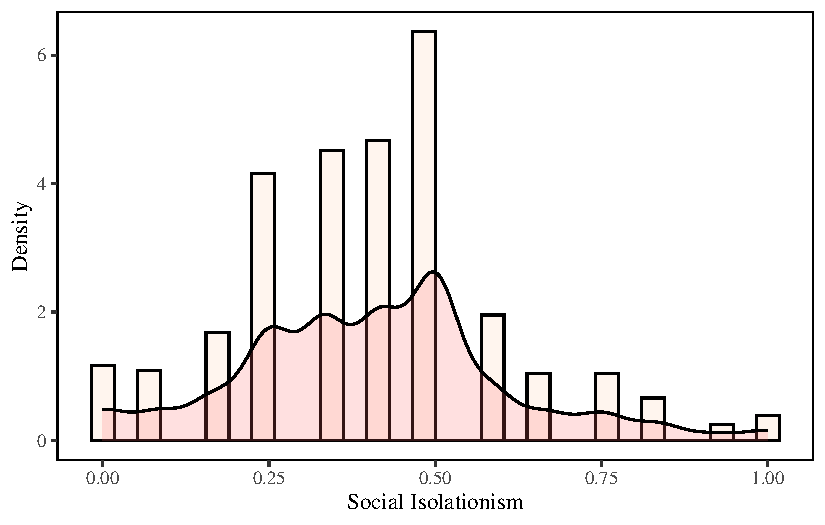
\includegraphics{Social-Isolation-in-China_files/figure-pdf/fig-social-iso-dist-1.pdf}

}

\caption{\label{fig-social-iso-dist}Distribution of Social Isolationism
Index}

\end{figure}

We have several primary independent variables including human
interaction, online to offline relationships, general social media use,
and urbanicity. We measured human interaction with a single item: ``Has
the internet and phone applications increased your contact with the
following groups of people (check yes to all that apply)?'' The response
options were: 1) Family that lives nearby, 2) Family that lives far
away, 3) Friends that live nearby, 4) Friends that live far away, 5)
People you met on the internet that live nearby, and 6) People you met
on the internet that live far away. We simply counted the number of
selected responses so the item ranged from 0 to 6, and then for the
models that come later, we rescaled it to range from 0 through 1
maintaining the original intervals. Online to offline relationships was
also measured with a single item: Have you met someone offline that you
initially met online? Response options were: 1) Yes, many times, 2) Yes,
several times, 3) Yes, once, and 4) No, never. We inverted this scale so
that higher values represented more offline relationships, and again,
rescaled it to range from 0 through 1 for the models that follow.

The distributions of these ordinal independent variables are reflected
in Figure~\ref{fig-var-dist}. Very few people claimed to never have
increased their contact/connections with others through the internet.
The modal number of increased connections respondents claimed to have
made through the internet was 2, followed closely by 1, but a sizable
proportion of the sample, about 48\% claimed to have increased their
number of personal connections by 3 or more through the internet.
Perhaps not surprisingly, the modal response when asked whether one had
met someone online and that relationship moved offline was ``No,
never''. On the other hand, we were surprised that about 37\% of those
sampled claimed to have moved relationships offline several times, over
10\% said they had done so many times, and about 13\% did so once. Taken
altogether, a large proportion of our respondents seem to using the
internet to facilitate social relations.

\begin{figure}

{\centering 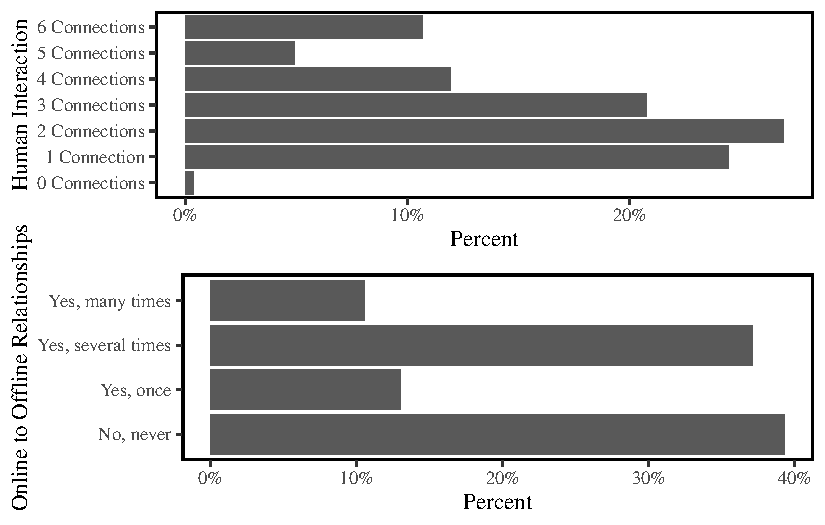
\includegraphics{Social-Isolation-in-China_files/figure-pdf/fig-var-dist-1.pdf}

}

\caption{\label{fig-var-dist}Primary Independent Variables
Distributions}

\end{figure}

We measured general social media use with an index based on the
following three items: 1) About how many hours a day would you estimate
you spend using only social media? Social media means applications like
Weibo, QQ, Renren, Kaixin001, Douban, WeChat or other sites and services
that allow users to interact with each other. (0-1, 1-2, 2-3, 3-4, 4-5,
5-6, 6-7, 7-8, 8-9, or More than 9), 2) Do you check email, read
websites, and use social media (social media means applications like
Weibo, QQ, Renren, Kaixin001, Douban, WeChat or other sites and services
that allow users to interact with each other) more than you did five
years ago? (Yes, No), and 3) How often do you read news stories about
political events that have been posted on social media (social media
means applications like Weibo, QQ, Renren, Kaixin001, Douban, WeChat or
other sites and services that allow users to interact with each other)?
(More than once a day, Everyday, Three-to-five days per week, One-to-two
days per week, Less often, Never). Each was recoded so that higher
values represented more social media use, rescaled to range from 0
through 1, added together, and then again, rescaled to range from 0
through 1 maintaining all original intervals. The distribution of this
index is presented in Figure~\ref{fig-sm-use-dist}. The distribution is
relatively normal and tightly centered around the mean 0.63 with a
standard deviation of 0.17, but there is a left skew suggesting that a
portion of the population is not that social media active, but clearly
the bulk of the population are.

\begin{figure}

{\centering 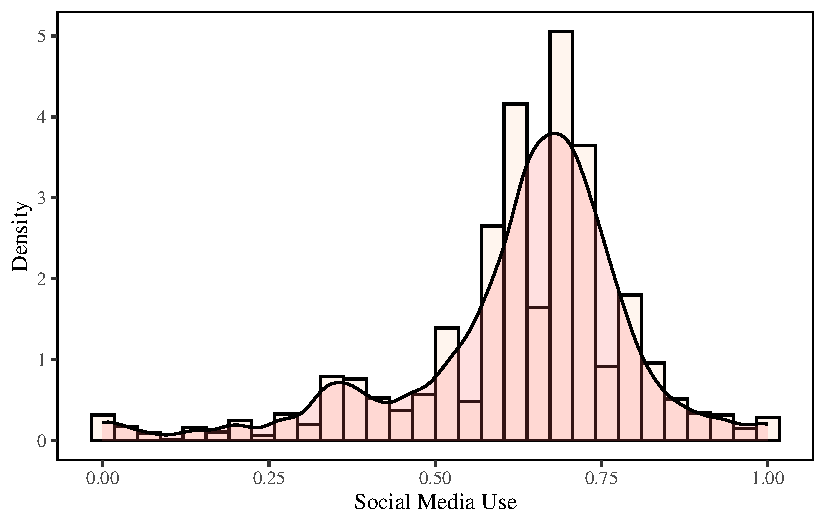
\includegraphics{Social-Isolation-in-China_files/figure-pdf/fig-sm-use-dist-1.pdf}

}

\caption{\label{fig-sm-use-dist}General Social Media Use Distribution}

\end{figure}

Our final primary independent variable, urbanicity, was measured using a
single item: Which of these best describes the place in which you live?
(Countryside/Village, Small City, Mid-Sized City, Suburban Area of a Big
City, Big City). For the purpose of the models, we rescaled this item to
range from 0 through 1 maintaining the original intervals. The
distribution is reflected in Figure~\ref{fig-urban-dist}. Given the
rural to urban Chinese migration since the founding of the People's
Republic (Xia, 1995), it is not surprising to see that nearly 45\% of
those in our sample live in cities, 7\% in suburbs, and about 27\% in
mid-sized cities. About 16\% say they live in small cities and only
about 5\% say they live in villages.

\begin{figure}

{\centering 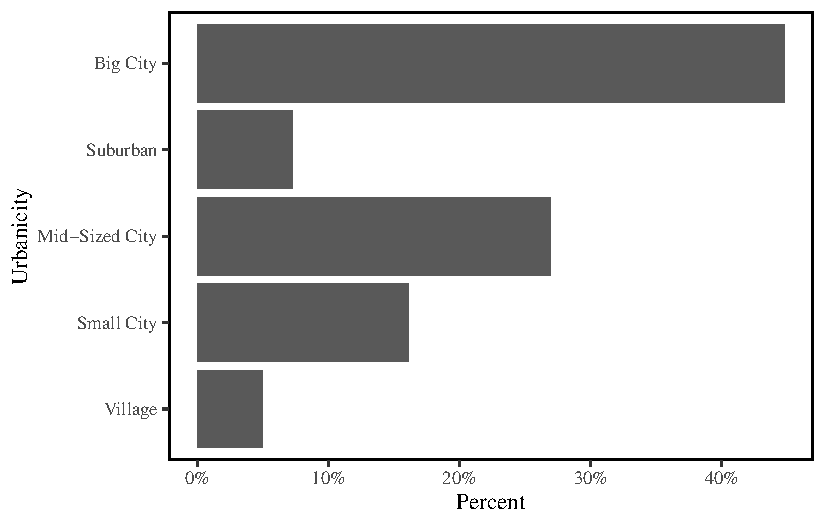
\includegraphics{Social-Isolation-in-China_files/figure-pdf/fig-urban-dist-1.pdf}

}

\caption{\label{fig-urban-dist}Urbanicity Distribution}

\end{figure}

Our modeling strategy that follows is straightforward. We begin by
modeling each of our internet communication independent variables as
function of socio-economic status (SES), gender, Chinese Communist Party
membership (CCP), and age to create an individual profile of each type
of digital user (see the Online Appendix for the operationalization of
these variables). This provides some context for the models that follow
which are intended to test our primary hypotheses, that is that internet
communication can deter social isolation and that this is particularly
true for those who do not have the convenience of the high social
interaction opportunity provided by urban living. For those we begin by
fitting an additive model of our index of social isolationism as
function of each of our primary independent variables while also
controlling for the same variables included in our profile models.
Finally, we refit three models with the same specification but introduce
an interactive term between each of our internet communication
indicators, respectively, with our measure of urbanicity. This allows us
to test whether the observed additive effects are stronger for those
living outside cities.

\hypertarget{results}{%
\subsection{Results}\label{results}}

Given that the first two dependent variables (human interaction, online
to offline to offline relationships) in our profile models are
distributed ordinally, we initially estimate linear models of those
outcomes and examine the residual behavior to determine if a linear
model fits the data well or if an ordered outcome model is a better fit.
The results were clear, a linear model is not a good fit for either
outcome (see the figures in the Online Appendix), so we fit the models
using ordered logit. Because our measure of general social media is
based on an additive index, we treat it as continuous, and accordingly
fit a linear model.

\hypertarget{tbl-profile-models}{}
\begin{table}
\caption{\label{tbl-profile-models}Modeling Profiles of Digital Communication }\tabularnewline

\centering
\begin{threeparttable}
\begin{tabular}[t]{lccc}
\toprule
  & Human Interaction & Online/Offline Interaction & General Social Media\\
\midrule
SES & \num{2.35}* & \num{2.16}* & \num{0.24}*\\
 & (\num{0.27}) & (\num{0.28}) & (\num{0.03})\\
Female & \num{-0.03} & \num{-0.35}* & \num{0.01}\\
 & (\num{0.08}) & (\num{0.08}) & (\num{0.01})\\
CCP Member & \num{-0.17} & \num{0.23}* & \num{0.01}\\
 & (\num{0.09}) & (\num{0.09}) & (\num{0.01})\\
Age & \num{0.51}* & \num{-0.82}* & \num{-0.12}*\\
 & (\num{0.26}) & (\num{0.27}) & (\num{0.02})\\
\midrule
N & \num{2277} & \num{2276} & \num{2198}\\
Pseudo R2 & \num{0.07} & \num{0.05} & \\
R2 &  &  & \num{0.05}\\
\bottomrule
\multicolumn{4}{l}{\rule{0pt}{1em}* p $<$ 0.05}\\
\end{tabular}
\begin{tablenotes}
\item \textit{Note: } 
\item Human Interaction and Offline/Online Relationships estimates are derived from ordered logit and General Social Media from ordinary least squares.
\end{tablenotes}
\end{threeparttable}
\end{table}

The results of our profile models are presented in
Table~\ref{tbl-profile-models}. When it comes to SES, the relationship
across all three of our internet communication is consistent. As SES
goes up so does digital human interaction, the move from online to
offline relationships, and general social media use. That gender is only
statistically significant in the model of the move from online to
offline relationships where women are less likely to do so.
Interestingly, being a CCP member has inverse relationships with human
interaction and the move from online to offline, where members are less
likely to increase digital human interaction but are more likely to move
online relationships offline. Finally, the older respondents were the
more likely they were to increase human interaction, and the less likely
they were to move relationships offline and use social media. These
profile results provide background context for the models that follow.
The internet communication indicators are our primary independent
variables, so these profile models give us a sense for whom they matter
the most when it comes to deterring social isolation.

\hypertarget{tbl-social-isolation-models}{}
\begin{table}
\caption{\label{tbl-social-isolation-models}Modeling Social Isolation }\tabularnewline

\centering
\begin{threeparttable}
\begin{tabular}[t]{lcccc}
\toprule
  & (1) & (2) & (3) & (4)\\
\midrule
Human Interaction & \num{-0.14}* & \num{-0.04} & \num{-0.14}* & \num{-0.14}*\\
 & (\num{0.02}) & (\num{0.04}) & (\num{0.02}) & (\num{0.02})\\
Online-Offline & \num{0.07}* & \num{0.07}* & \num{0.15}* & \num{0.07}*\\
 & (\num{0.01}) & (\num{0.01}) & (\num{0.03}) & (\num{0.01})\\
Social Media & \num{0.05}* & \num{0.05}* & \num{0.05}* & \num{0.13}*\\
 & (\num{0.03}) & (\num{0.02}) & (\num{0.02}) & (\num{0.05})\\
Urbanicity & \num{-0.04}* & \num{0.02} & \num{0.01} & \num{0.04}\\
 & (\num{0.01}) & (\num{0.03}) & (\num{0.02}) & (\num{0.05})\\
SES & \num{-0.04} & \num{-0.04} & \num{-0.04} & \num{-0.04}\\
 & (\num{0.03}) & (\num{0.03}) & (\num{0.03}) & \vphantom{1} (\num{0.03})\\
Female & \num{0.02}* & \num{0.02}* & \num{0.02}* & \num{0.02}*\\
 & (\num{0.01}) & (\num{0.01}) & (\num{0.01}) & \vphantom{1} (\num{0.01})\\
CCP Member & \num{0.00} & \num{0.00} & \num{0.00} & \num{0.00}\\
 & (\num{0.01}) & (\num{0.01}) & (\num{0.01}) & (\num{0.01})\\
Age & \num{-0.19}* & \num{-0.20}* & \num{-0.20}* & \num{-0.20}*\\
 & (\num{0.03}) & (\num{0.03}) & (\num{0.03}) & (\num{0.03})\\
Human Interaction*Urbanicity &  & \num{-0.14}* &  & \\
 &  & (\num{0.05}) &  & \\
Online-Offline*Urbanicity &  &  & \num{-0.12}* & \\
 &  &  & (\num{0.03}) & \\
Social Media*Urbanicity &  &  &  & \num{-0.13}\\
 &  &  &  & (\num{0.07})\\
\midrule
N & \num{2173} & \num{2173} & \num{2173} & \num{2173}\\
R2 & \num{0.08} & \num{0.08} & \num{0.09} & \num{0.08}\\
\bottomrule
\multicolumn{5}{l}{\rule{0pt}{1em}* p $<$ 0.05}\\
\end{tabular}
\begin{tablenotes}
\item \textit{Note: } 
\item Estimates are derived using ordinary least squares
\end{tablenotes}
\end{threeparttable}
\end{table}

The results of our models of social isolation are presented in
Table~\ref{tbl-social-isolation-models}. The additive estimates in model
(1) provide mixed results regarding whether internet communication is a
positive force in deterring social isolation. Not surprisingly, there is
a negative relationship between the number of digital connections (human
interaction) folks make and feelings of social isolation. On the other
hand, though, both moving online relationships offline and general
social media use are positively related to feelings of social isolation.
The latter is consistent with much of the literature outlined above, but
the former is not. Perhaps, this is context driven. The results also
indicate that those living in more urban environments tend to feel less
socially isolated.

Models (2) - (4) in Table 2 include each of the interactions between our
three internet communication measures and urbanicity. The consistent
result across the interactions is that the relationships are dulled for
those living in more rural areas. The interaction between digital humna
interaction and urbanicity is statistically significant (\(p < 0.01\)),
as is that between the move from online to offline relationships and
urbanicity (\(p < 0.001\)), and that between general social media use
and urbanicity only slightly misses the arbitrary \(0.05\) threshold
(\(p = 0.07\)). The interactions are most easily interpreted graphically
(see Figure~\ref{fig-social-isolation-interactions}).

\begin{figure}

{\centering 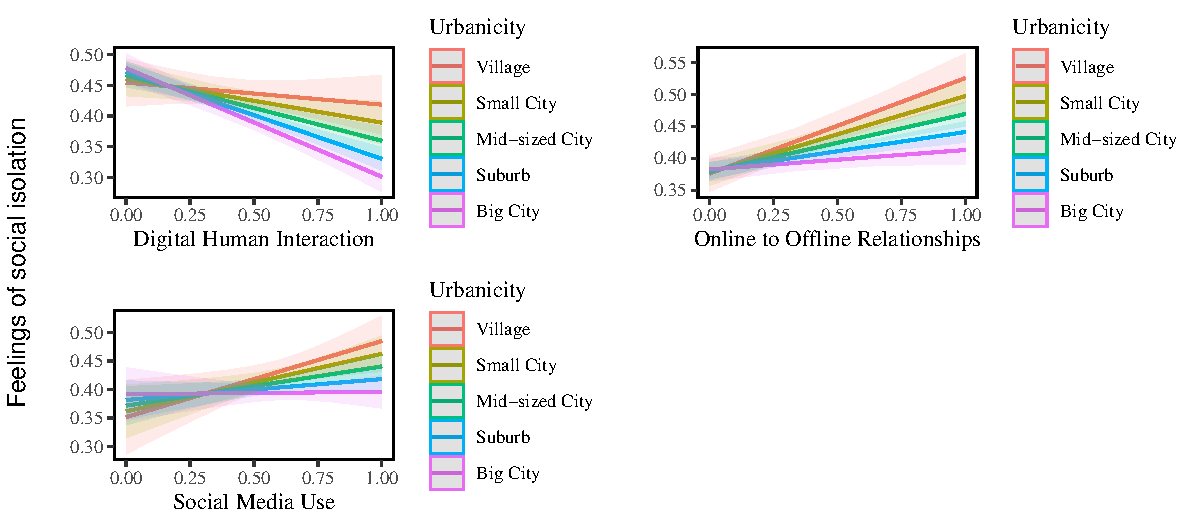
\includegraphics{Social-Isolation-in-China_files/figure-pdf/fig-social-isolation-interactions-1.pdf}

}

\caption{\label{fig-social-isolation-interactions}Modeling Social
Isolation: Interaction Results}

\end{figure}

The model (2) results are graphed in the upper left hand figure. Here it
is clear that the negative relationship between digital human
interaction and feelings of social isolation is considerably stronger
for those in cities. For that matter, notice that the relationship for
those in villages is basically flat; the 95 percent confidence interval
around the slight negative slope indicates that the relationship could
be flat.

The results from the interaction between online to offline relationships
and urbanicity are displayed in the graph in the upper right hand corner
of Figure 5. Again, here, the main effects run in the opposite direction
than those of digital human interaction. Those who are more likely to
move relationships from online to offline tend to feel more isolated,
and the interactive results presented here suggest that this relations
is stronger for those living in less urban spaces. Likewise, the same is
the case for those using social media more frequently. In fact, the
relationship here for those living in the largest cities is completely
non-existent.

In terms of our original hypotheses, we find support for the idea that
China's social media environment is not particularly unique with respect
to generating feelings of social isolation (\textbf{H1b}). Whether or
not this is due to the influencer culture or other factors, we cannot
say with our data but it at least does suggest that greater content
regulation is not likely to moderate the amount of isolation that social
media produces. We also find, as has been found in other studies, that
users who use the internet to create new connections are less likely to
feel isolated (\textbf{H2}). However, this does not seem to extend to
those that use the internet to facilitate offline meetups. Finally, we
find that the impact of the internet and social media vary significantly
according to the level of urbanicity (\textbf{H3}) - this matches with
previous findings that suggest that there is significant heterogeneity
in the impact of social media on social isloation. All of these findings
are generally in line with previous research on the subject, suggesting
that the mechanisms that generate feelings of social isolation are
universal and not so sensitive to different social and governing
contexts.

\hypertarget{conclusion}{%
\subsection{Conclusion}\label{conclusion}}

Cyberoptimists heralded the internet as means by which people could
connect, build social capital, and some suggested this could deter
social isolationism. Our results provide little evidence of this
optimistic view of the internet and its ability to improve the quality
of people's lives. We do find that some are more likely to interact with
family and friends and that this does deter feelings of social
isolation, but on the other hand, even though many move online
relationships offline and connect through social media, doing so does
not deter feelings of social isolation. Instead, such digital actively
is actually associated with increased feelings of social isolation.

We also found no evidence that the internet could serve as bridge to
build connections for those living outside of cities. The optimistic
view here would be that the internet could lower the costs of making
connections for those who have less social opportunity, those living in
less populated areas, and as a result, help them to feel less isolated.
We, in fact, found the opposite. Internet communication had either less
positive effect or more negative effect on feelings of social isolation
for those living in less urban spaces.

Our contribution here is that we look at some well-established
theoretical arguments in a context outside that of where most of the
research centered on these type questions has examined. While our study
is far from the last word on the subject, these results suggest that the
mechanisms that link social media use and social isolation are
relatively consistent across countries.

\newpage{}

\hypertarget{references}{%
\subsection{References}\label{references}}

\hypertarget{refs}{}
\begin{CSLReferences}{1}{0}
\leavevmode\vadjust pre{\hypertarget{ref-ademiluyi2022}{}}%
Ademiluyi A, Li C and Park A (2022)
\href{https://doi.org/10.2196/30286}{Implications and Preventions of
Cyberbullying and Social Exclusion in Social Media: Systematic Review}.
\emph{JMIR Formative Research} 6(1): e30286.

\leavevmode\vadjust pre{\hypertarget{ref-alabri2022}{}}%
Alabri A (2022) \href{https://doi.org/10.1155/2022/4824256}{Fear of
Missing Out (FOMO): The Effects of the Need to Belong, Perceived
Centrality, and Fear of Social Exclusion}. \emph{Human Behavior and
Emerging Technologies} 2022: e4824256.

\leavevmode\vadjust pre{\hypertarget{ref-appel2020}{}}%
Appel M, Marker C and Gnambs T (2020)
\href{https://doi.org/10.1177/1089268019880891}{Are Social Media Ruining
Our Lives? A Review of Meta-Analytic Evidence}. \emph{Review of General
Psychology} 24(1): 60--74.

\leavevmode\vadjust pre{\hypertarget{ref-beyens2020}{}}%
Beyens I, Pouwels JL, Driel II van, et al. (2020)
\href{https://doi.org/10.1038/s41598-020-67727-7}{The effect of social
media on well-being differs from adolescent to adolescent}.
\emph{Scientific Reports} 10(1): 10763.

\leavevmode\vadjust pre{\hypertarget{ref-buxfcttner2022}{}}%
Büttner CM and Rudert SC (2022)
\href{https://doi.org/10.1016/j.chb.2021.107062}{Why didn't you tag
me?!: Social exclusion from Instagram posts hurts, especially those with
a high need to belong}. \emph{Computers in Human Behavior} 127: 107062.

\leavevmode\vadjust pre{\hypertarget{ref-chinas2016}{}}%
China{'}s latest social media trend: Diaosi / loser subculture (2016).
Available at:
\url{https://www.appnova.com/chinas-latest-social-media-trend-diaosi-loser-subculture/}.

\leavevmode\vadjust pre{\hypertarget{ref-ellison2007}{}}%
Ellison NB, Steinfield C and Lampe C (2007)
\href{https://doi.org/10.1111/j.1083-6101.2007.00367.x}{The Benefits of
Facebook {``}Friends:{''} Social Capital and College Students{'} Use of
Online Social Network Sites}. \emph{Journal of Computer-Mediated
Communication} 12(4): 1143--1168.

\leavevmode\vadjust pre{\hypertarget{ref-hajek2019}{}}%
Hajek A and König H-H (2019)
\href{https://doi.org/10.1186/s12889-018-6369-6}{The association between
use of online social networks sites and perceived social isolation among
individuals in the second half of life: results based on a nationally
representative sample in Germany}. \emph{BMC Public Health} 19(1): 40.

\leavevmode\vadjust pre{\hypertarget{ref-henning-smith2018}{}}%
Henning-Smith C, Ecklund A and Kozhimannil K (2018)
\href{https://doi.org/10.1093/geroni/igy023.2851}{RURAL-URBAN
DIFFERENCES IN SOCIAL ISOLATION AND ITS RELATIONSHIP TO HEALTH}.
\emph{Innovation in Aging} 2(Suppl 1): 770.

\leavevmode\vadjust pre{\hypertarget{ref-kaye2017}{}}%
Kaye LW (2017) \href{https://doi.org/10.1093/ppar/prx029}{Older adults,
rural living, and the escalating risk of social isolation}. \emph{Public
Policy \& Aging Report} 27(4): 139--144.

\leavevmode\vadjust pre{\hypertarget{ref-kim2017}{}}%
Kim HH (2017) \href{https://doi.org/10.1080/02673843.2016.1197135}{The
impact of online social networking on adolescent psychological
well-being (WB): A population-level analysis of korean school-aged
children}. \emph{International Journal of Adolescence and Youth} 22(3):
364--376.

\leavevmode\vadjust pre{\hypertarget{ref-koning2017}{}}%
Koning JLD, Stathi A and Richards S (2017)
\href{https://doi.org/10.1017/S0144686X16000696}{Predictors of
loneliness and different types of social isolation of rural-living older
adults in the United Kingdom}. \emph{Ageing \& Society} 37(10):
2012--2043.

\leavevmode\vadjust pre{\hypertarget{ref-larson2018}{}}%
Larson LR, Szczytko R, Bowers EP, et al. (2018) Outdoor Time, Screen
Time, and Connection to Nature: Troubling Trends Among Rural Youth?
\emph{Environment and Behavior}. Epub ahead of print 20 October 2018.
DOI:
\href{https://doi.org/10.1177/0013916518806686}{10.1177/0013916518806686}.

\leavevmode\vadjust pre{\hypertarget{ref-li2017}{}}%
Li J and Rose N (2017)
\href{https://doi.org/10.1016/j.healthplace.2017.08.009}{Urban social
exclusion and mental health of China's rural-urban migrants
{\textendash} A review and call for research}. \emph{Health \& Place}
48: 20--30.

\leavevmode\vadjust pre{\hypertarget{ref-lim2020}{}}%
Lim MH, Eres R and Vasan S (2020)
\href{https://doi.org/10.1007/s00127-020-01889-7}{Understanding
loneliness in the twenty-first century: An update on correlates, risk
factors, and potential solutions}. \emph{Social Psychiatry and
Psychiatric Epidemiology} 55(7): 793--810.

\leavevmode\vadjust pre{\hypertarget{ref-liu2020}{}}%
Liu C and Liu Y (2020)
\href{https://doi.org/10.3390/ijerph17134720}{Media Exposure and Anxiety
during COVID-19: The Mediation Effect of Media Vicarious
Traumatization}. \emph{International Journal of Environmental Research
and Public Health} 17(13): 4720.

\leavevmode\vadjust pre{\hypertarget{ref-liu2022}{}}%
Liu J and Yang L (2022)
\href{https://doi.org/10.1002/poi3.307}{{``}Dual-Track{''} platform
governance on content: A comparative study between China and United
States}. \emph{Policy \& Internet} 14(2): 304--323.

\leavevmode\vadjust pre{\hypertarget{ref-nan2013}{}}%
Nan W (2013)
\href{https://www.scmp.com/news/china/article/1232976/chinas-underdog-youth-find-success-diaosi-or-loser-identity}{China's
underdog youth find success in 'diaosi' - or 'loser' - identity}.
\emph{South China Morning Post}. Epub ahead of print 8 May 2013.

\leavevmode\vadjust pre{\hypertarget{ref-nowland2018}{}}%
Nowland R, Necka EA and Cacioppo JT (2018)
\href{https://doi.org/10.1177/1745691617713052}{Loneliness and Social
Internet Use: Pathways to Reconnection in a Digital World?}
\emph{Perspectives on Psychological Science} 13(1): 70--87.

\leavevmode\vadjust pre{\hypertarget{ref-ostic2021}{}}%
Ostic D, Qalati SA, Barbosa B, et al. (2021)
\href{https://www.frontiersin.org/articles/10.3389/fpsyg.2021.678766}{Effects
of social media use on psychological well-being: A mediated model}.
\emph{Frontiers in Psychology} 12.

\leavevmode\vadjust pre{\hypertarget{ref-primack2017}{}}%
Primack BA, Shensa A, Sidani JE, et al. (2017)
\href{https://doi.org/10.1016/j.amepre.2017.01.010}{Social Media Use and
Perceived Social Isolation Among Young Adults in the U.S.}
\emph{American Journal of Preventive Medicine} 53(1): 1--8.

\leavevmode\vadjust pre{\hypertarget{ref-steinfield2008}{}}%
Steinfield C, Ellison NB and Lampe C (2008)
\href{https://doi.org/10.1016/j.appdev.2008.07.002}{Social capital,
self-esteem, and use of online social network sites: A longitudinal
analysis}. \emph{Journal of Applied Developmental Psychology} 29(6).
Social Networking on the Internet: 434--445.

\leavevmode\vadjust pre{\hypertarget{ref-subrahmanyam2008}{}}%
Subrahmanyam K, Reich SM, Waechter N, et al. (2008)
\href{https://doi.org/10.1016/j.appdev.2008.07.003}{Online and offline
social networks: Use of social networking sites by emerging adults}.
\emph{Journal of Applied Developmental Psychology} 29(6). Social
Networking on the Internet: 420--433.

\leavevmode\vadjust pre{\hypertarget{ref-szablewicz2014}{}}%
Szablewicz M (2014) \href{https://doi.org/10.1177/0920203X14531538}{The
{`}losers{'} of China{'}s Internet: Memes as {`}structures of feeling{'}
for disillusioned young netizens}. \emph{China Information} 28(2):
259--275.

\leavevmode\vadjust pre{\hypertarget{ref-tam2019}{}}%
Tam L (2019)
\href{https://www.scmp.com/lifestyle/entertainment/article/2183174/trust-me-you-need-how-chinas-live-streaming-kol-stars-are}{The
China fame factory training online influencers to sell}. \emph{South
China Morning Post}. Epub ahead of print 24 January 2019.

\leavevmode\vadjust pre{\hypertarget{ref-twenge2019}{}}%
Twenge JM (2019) \href{https://doi.org/10.1177/0963721419838244}{More
Time on Technology, Less Happiness? Associations Between Digital-Media
Use and Psychological Well-Being}. \emph{Current Directions in
Psychological Science} 28(4): 372--379.

\leavevmode\vadjust pre{\hypertarget{ref-twenge2017}{}}%
Twenge JM, Krizan Z and Hisler G (2017)
\href{https://doi.org/10.1016/j.sleep.2017.08.013}{Decreases in
self-reported sleep duration among U.S. adolescents
2009{\textendash}2015 and association with new media screen time}.
\emph{Sleep Medicine} 39: 47--53.

\leavevmode\vadjust pre{\hypertarget{ref-twenge2021}{}}%
Twenge JM, Haidt J, Blake AB, et al. (2021)
\href{https://doi.org/10.1016/j.adolescence.2021.06.006}{Worldwide
increases in adolescent loneliness}. \emph{Journal of Adolescence} 93:
257--269.

\leavevmode\vadjust pre{\hypertarget{ref-valkenburg2022}{}}%
Valkenburg PM, Meier A and Beyens I (2022)
\href{https://doi.org/10.1016/j.copsyc.2021.08.017}{Social media use and
its impact on adolescent mental health: An umbrella review of the
evidence}. \emph{Current Opinion in Psychology} 44: 58--68.

\leavevmode\vadjust pre{\hypertarget{ref-wang2020}{}}%
Wang J (2020) \emph{Regulation of digital media platforms: The case of
china}. 6 November. Foundation for Law, Justice,; Society. Available at:
\url{https://www.fljs.org/banning-regulating-tiktok-addressing-concerns-national-security-privacy-and-online-harms}.

\leavevmode\vadjust pre{\hypertarget{ref-wei2023}{}}%
Wei AC (2023)
\href{https://www.straitstimes.com/asia/east-asia/wang-hong-culture-booms-in-china-as-more-young-people-dream-of-becoming-influencers}{{`}Wang
hong{'} culture booms in China as more young people dream of becoming
influencers}. \emph{The Straits Times}. Epub ahead of print 27 May 2023.

\leavevmode\vadjust pre{\hypertarget{ref-xia1995}{}}%
Xia M (1995) Changes in the {Pattern} of {Migration} in {Urban} {China}.
In: Day LH, Xia M, and Xia M (eds) \emph{Migration and {Urbanization} in
{China}}. New York, NY: Routledge.

\end{CSLReferences}

\newpage{}

\hypertarget{online-appendix}{%
\subsection{Online Appendix}\label{online-appendix}}

\hypertarget{variable-operationalization}{%
\subsubsection{Variable
Operationalization}\label{variable-operationalization}}

SES is an additive index of these two questions regarding income and
education. Each of the following questions were rescaled to range from 0
through 1, then the two questions were summed, and then rescaled to
range from 0 through 1 again.

\begin{itemize}
\item
  Here is a table showing the range of monthly incomes that people have.
  Which of the letters on this table best represents the total monthly
  income of your household (after tax)?

  \begin{itemize}
  \item
    0 - 3,000,
  \item
    3,000 - 6,000,
  \item
    6,000 - 10,000,
  \item
    10,000 - 15,000,
  \item
    15,000 - 25,000,
  \item
    25,000 - 40,000,
  \item
    More than 40,000
  \end{itemize}
\item
  What is the highest level of education that you have obtained?

  \begin{itemize}
  \item
    No formal education,
  \item
    Primary,
  \item
    Middle school,
  \item
    High school,
  \item
    University,
  \item
    Advanced Studies/Graduate School
  \end{itemize}
\end{itemize}

Other important predictor variables are operationalized as follows:

\begin{itemize}
\item
  Gender

  \begin{itemize}
  \item
    0 = male,
  \item
    1 = female
  \end{itemize}
\item
  Are you a member or probationary member of the CCP?

  \begin{itemize}
  \item
    0 = no,
  \item
    1 = yes
  \end{itemize}
\item
  How old are you? (rescaled to range from 0 through 1)
\end{itemize}

\newpage{}

\hypertarget{residual-analysis}{%
\subsubsection{Residual Analysis}\label{residual-analysis}}

\begin{figure}

{\centering 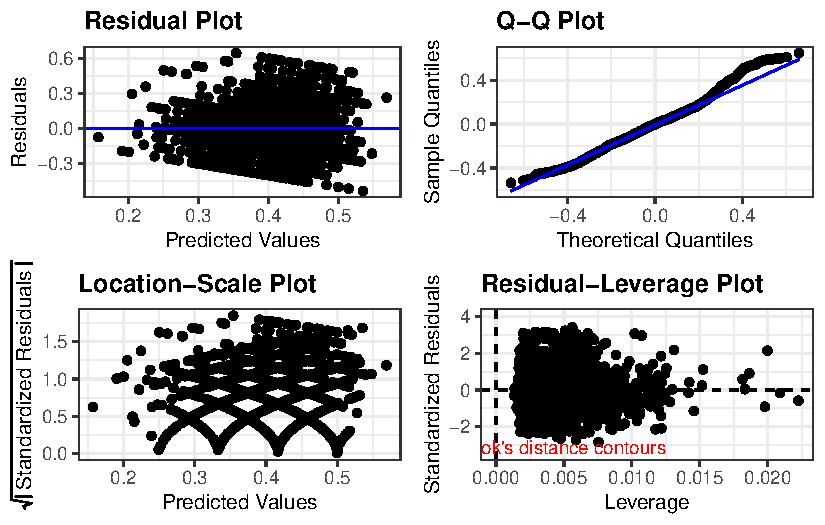
\includegraphics{Social-Isolation-in-China_files/figure-pdf/fig-resids-human-1.pdf}

}

\caption{\label{fig-resids-human}Human Interaction Model Residuals}

\end{figure}

\begin{figure}

{\centering 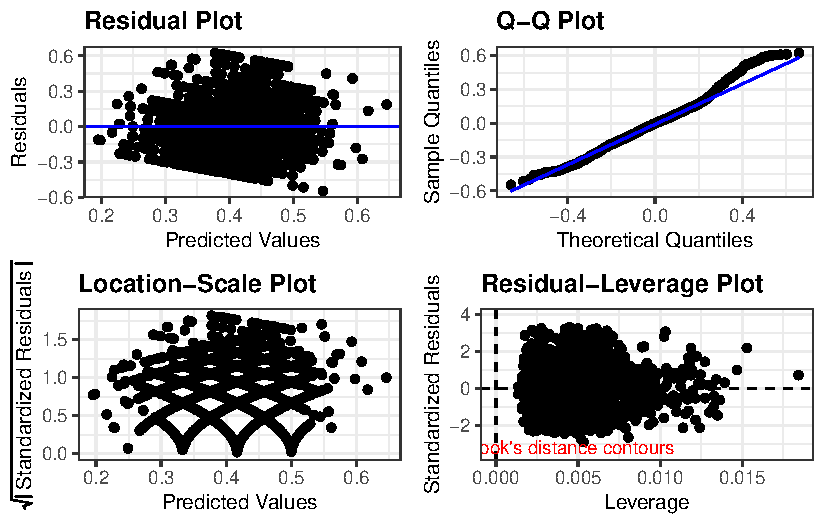
\includegraphics{Social-Isolation-in-China_files/figure-pdf/fig-resids-online-offline-1.pdf}

}

\caption{\label{fig-resids-online-offline}Online/Offline Model
Residuals}

\end{figure}



\end{document}
